\subsection{Изучение спектра атома водорода}

\paragraph{Экспериментальная установка}
Для измерения длин волн спектральных линий в работе используется
стеклянно-призменный монохроматор-спектрометр УМ-2 (универсальный монохроматор),
предназначенный для спектральных исследований в диапазоне от $0.38$ до $1.00$
мкм.


Основные элементы монохроматора представлены на рис. \ref{img::scheme}
\begin{figure}[h!]
  \centering
  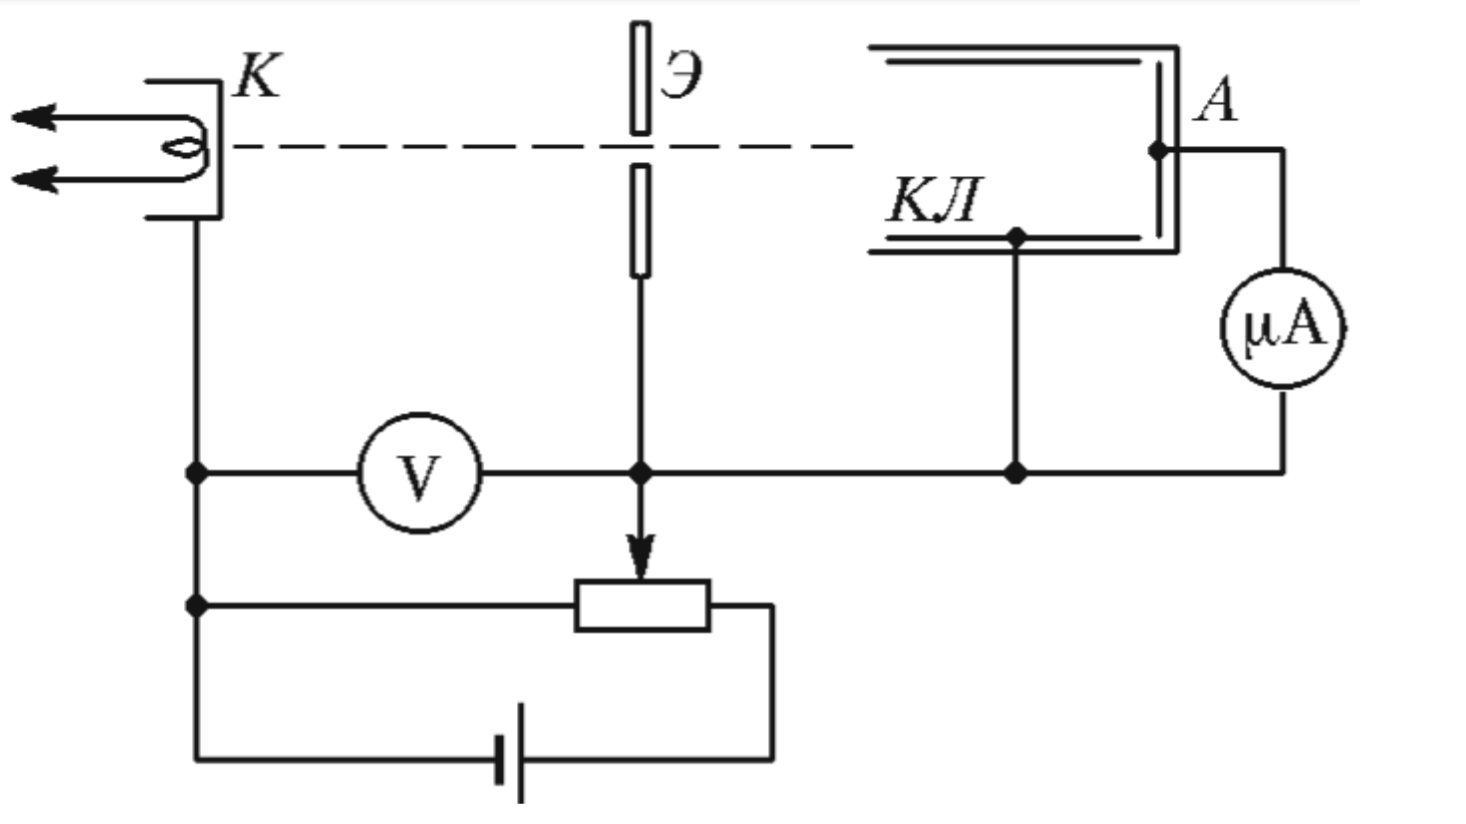
\includegraphics[width=0.5\linewidth]{scheme.png}
  \caption{Схема экспериментальной установки}
  \label{img::scheme}
\end{figure}


\begin{enumerate}
  \item Входная щель $1$, снабжённая микрометрическим винтом $9$, который
        позволяет открывать щель на нужную ширину (в диапазоне $0.01-4$ мм).
  \item Коллиматорный объектив $2$, снабжённый микрометрическим винтом $8$. Винт
        позволяет смещать объектив относительно щели при фокусировке спектральных
        линий различных цветов.
  \item Сложная спектральная призма $3$, установленная на поворотном столике
        $6$. Призма $3$ состоит из трёх склеенных призм $\Pi_1, \Pi_2$ и
        $\Pi_3$. Первые две призмы с преломляющими углами $30^{\circ}$
        изготовлены из тяжелого флинта, обладающего большой дисперсией.
        Промежуточная призма $\Pi_3$ сделана из крона. Лучи отражаются от её
        гипотенузной грани и поворачиваются на $90^{\circ}$. Благодаря такому
        устройству дисперсии призм $\Pi_1$ и $\Pi_2$ складываются.
  \item Поворотный столик $6$, вращающийся вокруг вертикальной оси при помощи
        микрометрического винта $7$ с отсчётным барабаном. На барабан нанесена
        винтовая дорожка с градусными делениями. Вдоль дорожки скользит указатель
        барабана. При вращении барабана призма поворачивается, и в центре поля зрения
        появляются различные участки спектра.
  \item Зрительная труба, состоящая из объектива $4$ и окуляра $5$. Объектив
        даёт изображение входной щели $1$ различных цветов в своей фокальной
        плоскости. В этой же плоскости расположено остриё указателя $10$. Изображение
        щели рассматривается через окуляр $5$. В случае необходимости окуляр может
        быть заменён выходной щелью, пропускающей всего одну из линий спектра ~---~
        тогда прибор служит монохроматором. В нашей работе выходная щель не
        применяется, то есть прибор используется как спектрометр.
  \item Массивный корпус $11$, предохраняющий прибор от повреждений и
        загрязнений.
  \item Оптическая скамья, на которой могут перемещаться рейтеры с источником
        света Л и конденсором К, служащим для концентрации света на входной щели.
        Входная щель спектрометра, конденсор и источник должны быть на одной высоте.
        Проходящий через входную щель световой пучок хорошо заполняет конденсор и
        призму, если выполнено соотношение $\frac{D_k}{b} = \frac{D_2}{f_2} =
          \frac{1}{6}$, где $D_k$ -- диаметр конденсора, $b$ -- расстояние от конденсора
        до входной щели, $D_2$ и $f_2$ -- диаметр и фокусное расстояние коллиматорного
        объектива $2$.

        Изображение удобно наблюдать на колпачке с крестиком (таким колпачком прикрывают щель при юстировке системы).
  \item Пульт управления (на рис. \ref{img::scheme} не показан), служащий для
        питания источников света и осветительной системы спектрометра. На пульте
        имеются гнёзда для подключения осветителей ($3.5$ В), неоновой лампы и лампы
        накаливания. Тумблеры, расположенные на основании спектрометра, позволяют
        включать лампочки осветителей шкал и указателя спектральных линий. Яркость
        освещения указателя регулируется реостатом.
\end{enumerate}

При подготовке УМ-2 к наблюдениям особое внимание следует обращать на тщательную
фокусировку, с тем чтобы указатель $10$ и спектральные линии имели чёткие, ясные
границы. Фокусировка производится в следующем порядке. Перемещая окуляр, следует
получить резкое изображение острия указателя $10$. Осветив входную щель прибора
ртутной лампой, нужно найти одну из спектральных линий и получить её резкое
изображение при помощи микрометрического винта $8$. При проведении измерений в
другой части спектра, последняя операция по фокусировке должна проводится вновь.

Для отсчёта положения спектральной линии её центр совмещается с остриём
указателя. Отсчёт производится по делениям барабана. Для уменьшения ошибки
ширину входной щели делают по возможности малой ($0.05-0.07$ мм по
микрометрической шкале). Для наблюдения самых слабых линий в крайней фиолетовой
области щель приходится несколько расширять. Глаз лучше замечает слабые линии в
движении, поэтому при наблюдении полезно слегка поворачивать барабан в обе
стороны от среднего положения.

Спектрометр УМ-2 нуждается в предварительной градуировке. Для градуировки в
коротковолновой части спектра удобно применять ртутную лампу ПРК-4, а в
длинноволновой и средней частях спектра ~---~ неоновую лампу. Таблицы
спектральных линий ртути и неона с визуальной оценкой их относительной
интенсивности приведены на установке.

\paragraph{Водородная лампа}
В опытах по измерению длин волн бальмеровской серии источником света служит
водородная трубка Н-образной формы, питаемая от источника высокого напряжения.
Наибольшая яркость спектра достигается в том случае, когда источником света
служит торец горизонтальной части трубки-капилляра (перемычки в букве Н).

Для увеличения яркости интересующих нас линий атомарного водорода в состав газа,
которым заполняют трубку при её изготовлении, добавляют пары воды. Молекулы воды
в электрическом разряде разлагаются, образуя атомарный водород. Трубка
заполняется до давления $5-10$ Торр.

Следует отметить, что в спектре водородной лампы наряду с линиями атомного
спектра наблюдается также спектр молекулярного водорода. Однако интенсивность
молекулярных линий значительно слабее и отождествление ярких атомных линий на
фоне молекулярного спектра не представляет большого труда.

\subsection{Изучение молекулярного спектра йода}

Молекулярный спектр поглощения паров йода можно наблюдать, используя

\begin{enumerate}
  \item источник сплошного спектра -- лампу накаливания;
  \item поглощаемую среду -- кювету с исследуемым веществом;
  \item спектральный прибор, регистрирующий спектр поглощения -- монохроматор
  УМ-2.
\end{enumerate}

\begin{figure}[h!]
  \centering
  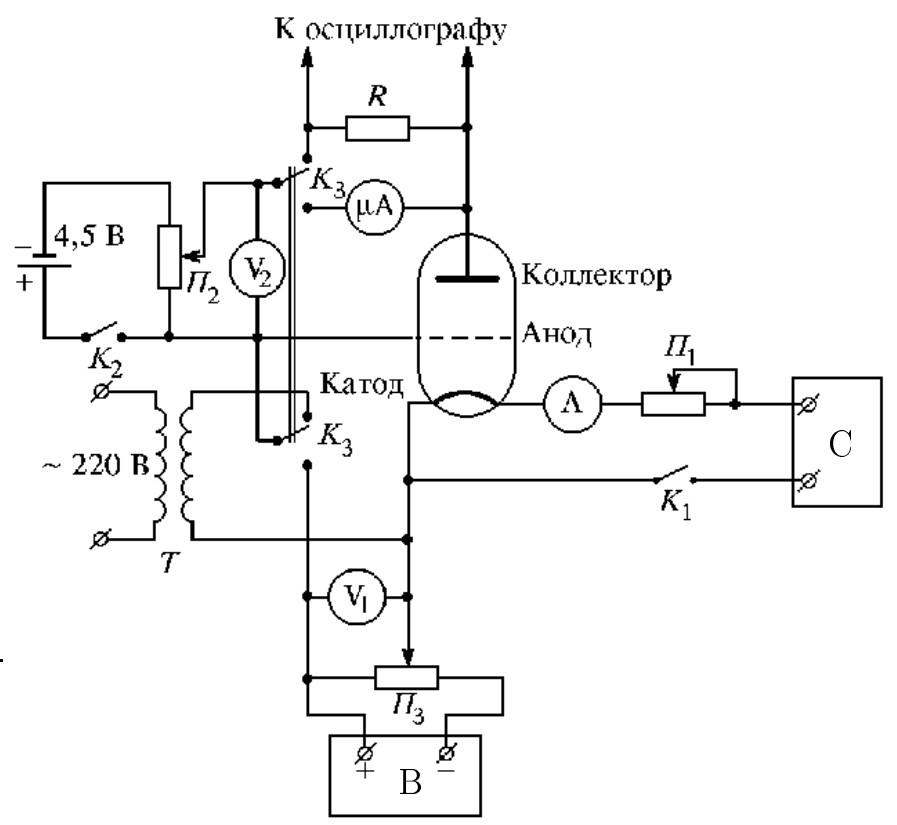
\includegraphics[width=0.9\linewidth]{pic3.png}
  \caption{Градуировка спектрометра}
  \label{pic3}
\end{figure}

В нашей работе спектр поглощения паров йода наблюдается визуально на фоне
сплошного спектра лампы накаливания $1$, питаемой от блока питания 2 (рис.
\ref{pic3}.)

Кювета $3$ с кристаллами йода подогревается нихромовой спиралью, подключенной
вместе с лампой накаливания к блоку питания. Линза $4$ используется как
конденсор.

\begin{figure}[h!]
  \centering
  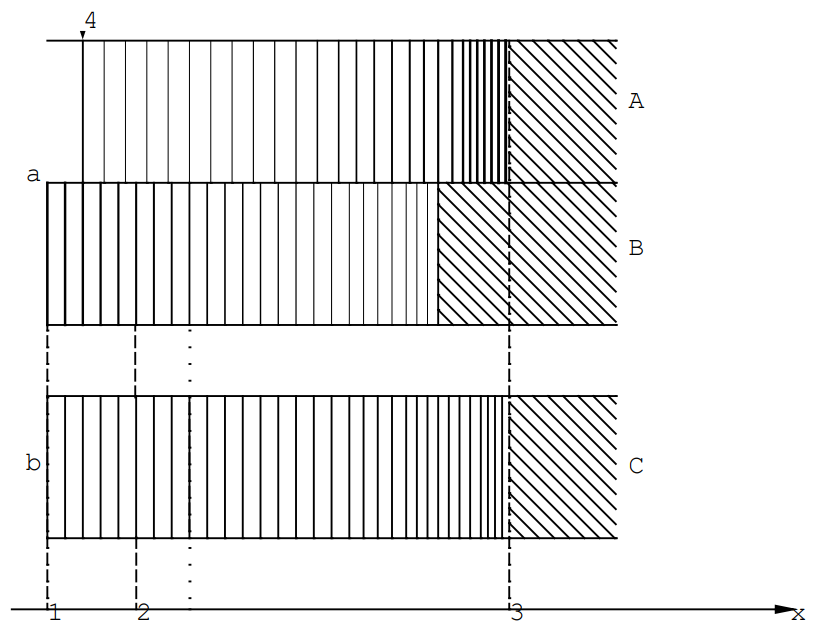
\includegraphics[width=0.9\linewidth]{pic4.png}
  \caption{Градуировка спектрометра}
  \label{pic4}
\end{figure}

В результате подогрева кристаллы йода частично возгоняются, образуя пары с
легкой фиолетовой окраской. Спектрометр позволяет визуально наблюдать линии
поглощения молекул йода на фоне сплошного спектра излучения лампы накаливания
видимой области (рис. \ref{pic4}.)
